\documentclass{beamer}
% ------------- START SETTINGS -------------------------------
%\documentclass[conference]{IEEEtran}
% \documentclass[11pt,twoside,a4paper]{article}
% \usepackage{blindtext, graphicx}

%\ifCLASSINFOpdf
%\else
%\fi

% A couple of useful packages
\usepackage[table]{xcolor}
\usepackage{listings}
\usepackage{color}
\usepackage{graphics} % for pdf, bitmapped graphics files
\usepackage{epsfig} % for postscript graphics files
\usepackage{mathptmx} % assumes new font selection scheme installed
\usepackage{times} % assumes new font selection scheme installed
\usepackage{amsmath} % assumes amsmath package installed
\usepackage{amssymb}  % assumes amsmath package installed
\usepackage{mdwmath}
\usepackage{algorithm}
\usepackage{algorithmic}
\usepackage{multirow}
\usepackage[margin=0.9in]{geometry}
%\usepackage[noend]{algpseudocode}


%\addbibresource{biblatex-ela427.bib}
% Added suport for bibtext files.
% \usepackage[backend=biber, sorting=none]{biblatex}
% --- packages for drawing diagrams----
\usepackage{tikz}
\usetikzlibrary{arrows,automata}


% Package that forces figures to stay within the section.
\usepackage[section]{placeins}

%package for utf-8 support
\usepackage[utf8]{inputenc}

% added support for bloc quotes
\usepackage{csquotes}

%colour
\usepackage{color}
%\graphicspath{ {images/}{mesurment/data} }

%Captions
%\usepackage[justification=centering,font=small,labelfont=bf]{caption}
\usepackage{hyperref}
\usepackage{url}

% New over line for inverse logic
%\newcommand{\overbar}[1]{\mkern 1.5mu\overline{\mkern-1.5mu#1\mkern-1.5mu}\mkern 1.5mu}
%\setcounter{secnumdepth}{3}

% -- Panda lines needed for DataFrame to latex ---
%\newcommand{\toprule}{\hline}
%\newcommand{\midrule}{\hline}
%\newcommand{\bottomrule}{\hline}
\usepackage[pages=some,scale=1,angle=0,opacity=0.7]{background}
\newcommand\BackImage[2][scale=1]{%
%\BgThispage
\backgroundsetup{
  contents={\includegraphics[#1]{#2}}
  }
}

% Renew the indexingsystem for sections, subsections, and subsubsections so that arabic numberalsare used - Added by Ulrik
\renewcommand{\thesection}{\arabic{section}}
\renewcommand{\thesubsection}{\thesection.\arabic{subsection}}
\def\thesectiondis{\thesection.} \def\thesubsectiondis{\thesectiondis\arabic{subsection}.} \def\thesubsubsectiondis{\thesubsectiondis\arabic{subsubsection}.} \def\theparagraphdis{\thesubsubsectiondis\arabic{paragraph}.}

% Among other things, allows for items to be bold - Added by Ulrik
\usepackage{enumitem}

\usepackage{cite}
% Imported ragged for justefiing text in the \who statement
\usepackage{ragged2e}
% cite.sty was written by Donald Arseneau
\usepackage{lipsum}
\usepackage{tabularx,ragged2e,booktabs}
\newcolumntype{C}[1]{>{\Centering}m{#1}}
\renewcommand\tabularxcolumn[1]{C{#1}}
% \usepackage{multirow}
%\usepackage{longtable}
% \usepackage{supertabular,booktabs}
% V1.6 and later of IEEEtran pre-defines the format of the cite.sty package
% \cite{} output to follow that of IEEE. Loading the cite package will
% result in citation numbers being automatically sorted and properly
% "compressed/ranged". e.g., [1], [9], [2], [7], [5], [6] without using
% cite.sty will become [1], [2], [5]--[7], [9] using cite.sty. cite.sty's
% \cite will automatically add leading space, if needed. Use cite.sty's
% noadjust option (cite.sty V3.8 and later) if you want to turn this off.
% cite.sty is already installed on most LaTeX systems. Be sure and use
% version 4.0 (2003-05-27) and later if using hyperref.sty. cite.sty does
% not currently provide for hyperlinked citations.
% The latest version can be obtained at:
% http://www.ctan.org/tex-archive/macros/latex/contrib/cite/
% The documentation is contained in the cite.sty file itself.


\setcounter{tocdepth}{1}

\usepackage[justification=centering, font=small, labelfont=bf]{caption}
\captionsetup[table]{name=Table}
\newcommand{\fs}[3]{\item \textbf{#1} ($#2\text{TiB} | #3\text{TiB}$) }
\newcommand{\fsE}[3]{\item \textbf{#1} ($#2\text{TiB} | #3\text{EiB}$) }
\newcommand{\fsEE}[3]{\item \textbf{#1} ($#2\text{EiB} | #3\text{EiB}$) }
\newcommand{\fsEZ}[3]{\item \textbf{#1} ($#2\text{EiB} | #3\text{ZiB}$) }

 % Programming color don't touch without permissions.
\definecolor{codegreen}{rgb}{0,0.6,0}
\definecolor{codeblue}{HTML}{0073e6}
\definecolor{codereed}{HTML}{fc0511}
\definecolor{codegray}{rgb}{0.4,0.4,0.4}
\definecolor{codeblac}{rgb}{0.9,0.9,0.9}
\definecolor{commentgray}{rgb}{0.7,0.7,0.7}
\definecolor{codepurple}{HTML}{3ad0d8}
\definecolor{stringblue}{HTML}{0073e6}
\definecolor{stringpurple}{HTML}{ff99ff}
\definecolor{stringgray}{rgb}{0.6,0.6,0.6}
\definecolor{backcolour}{rgb}{1,1,1}
\definecolor{graybackcolour}{rgb}{0.9,0.9,0.9}

\lstdefinestyle{bashStyle}{
    backgroundcolor=\color{graybackcolour},
    commentstyle=\color{commentgray},
    keywordstyle=\color{codeblue},
    numberstyle=\tiny\color{stringblue},
    stringstyle=\color{codegreen},
    basicstyle=\normalsize,
    breakatwhitespace=false,
    breaklines=true,
    captionpos=b,
    keepspaces=true,
    numbers=left,
    numbersep=4pt,
    showspaces=false,
    showstringspaces=false,
    showtabs=false,
    tabsize=4
}

\definecolor{pythonBG}{HTML}{f7faf2}

\lstdefinestyle{pythonStyle}{
    backgroundcolor=\color{pythonBG},
    commentstyle=\color{commentgray},
    keywordstyle=\color{codereed},
    numberstyle=\tiny\color{codepurple},
    stringstyle=\color{codegreen},
    basicstyle=\footnotesize,
    breakatwhitespace=false,
    breaklines=true,
    captionpos=b,
    keepspaces=true,
    numbers=left,
    numbersep=4pt,
    showspaces=false,
    showstringspaces=false,
    showtabs=false,
    tabsize=4
}

\definecolor{codegreen}{rgb}{0,0.6,0}
\definecolor{codegray}{rgb}{0.5,0.5,0.5}
\definecolor{codepurple}{rgb}{0.58,0,0.82}
\definecolor{backcolour}{rgb}{0.95,0.95,0.92}

\lstdefinestyle{textStyle}{
    backgroundcolor=\color{backcolour},
    commentstyle=\color{codegreen},
    keywordstyle=\color{magenta},
    numberstyle=\tiny\color{codegray},
    stringstyle=\color{codepurple},
    basicstyle=\footnotesize,
    breakatwhitespace=false,
    breaklines=true,
    captionpos=b,
    keepspaces=true,
    numbers=left,
    numbersep=4pt,
    showspaces=false,
    showstringspaces=false,
    showtabs=false,
    tabsize=4
}

\definecolor{bginstructions}{HTML}{e6f7ff}

\lstdefinestyle{instructStyle}{
    backgroundcolor=\color{bginstructions},
    numberstyle=\tiny\color{codegray},
    breakatwhitespace=false,
    breaklines=true,
    captionpos=b,
    keepspaces=true,
    numbers=left,
    numbersep=4pt,
    showspaces=false,
    showstringspaces=false,
    showtabs=false,
    tabsize=4
}



%\lstset{style=mystyle}
\lstdefinestyle{bash} {language=bash,style=bashStyle}
\lstdefinestyle{python} {language=Python,style=pythonStyle, morekeywords={with, as}}
\lstdefinestyle{python_style} {language=Python,style=pythonStyle, morekeywords={with, as}}
\lstdefinestyle{gcc} {language=c,style=bashStyle}
\lstdefinestyle{text} {style=textStyle, frame=lines}
\lstdefinestyle{instruct} {style=instructStyle, frame=lines, numbers=none}



\newcommand{\fsRAM}[1]{\item \textbf{#1} (nan$|$nan) }

\newcommand{\si}[1]{$(#1)$}
\usetheme{Boadilla}
% \usetheme{Madrid}


\usepackage[utf8]{inputenc}
\title{Using High Density Conductive
Polyethylene Black Foam as a restive sensor to
build spatial object awareness in robotic grippers}
\author{Magnus Sörensen, Daniel Stenekap}
\institute{Märlardalens högskola}
\date{2019}
\begin{document}
\frame{\titlepage}


\begin{frame}
    \begin{itemize}
        \item What is done.
        \item How it is done.
    \end{itemize}
\end{frame}

\begin{frame}
    \frametitle{Introduction}

    \begin{center}
        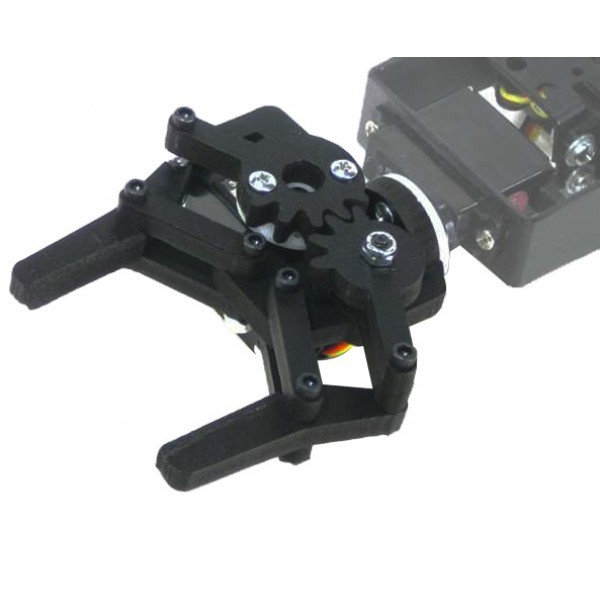
\includegraphics[width=.5\textwidth]{img/rob0078.jpg}
    \end{center}
    % #doc .NH
    % #doc Introduction
    % #doc .PP
    % #doc The most common robot gripper is as in this picture. Two flat often metal sheets pressing down on the
    % #doc tool it try to grab. No information on the shape, texture or features.
    % #doc In this work an attempt to create an sensor that could give robots an way to 'feel'
\end{frame}

\begin{frame}
    \frametitle{High Density Conductive
Polyethylene Black Foam}
    What is High Density Conductive Polyethylene Black Foam?
    \begin{center}
        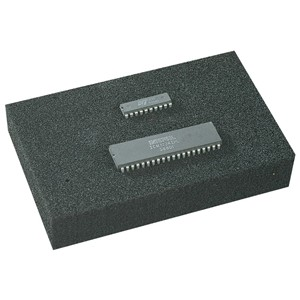
\includegraphics[width=.5\textwidth]{img/foam.jpg}
    \end{center}
    % #doc .NH
    % #doc Conductive foam.
    % #doc .PP
    % #doc What is  What is High Density Conductive Polyethylene Black Foam you might wonder.
    % #doc That foam is the foam you use to protect the Integrated circuits from static electricity.

\end{frame}

\begin{frame}
    \frametitle{How does it work?}
    \begin{center}
        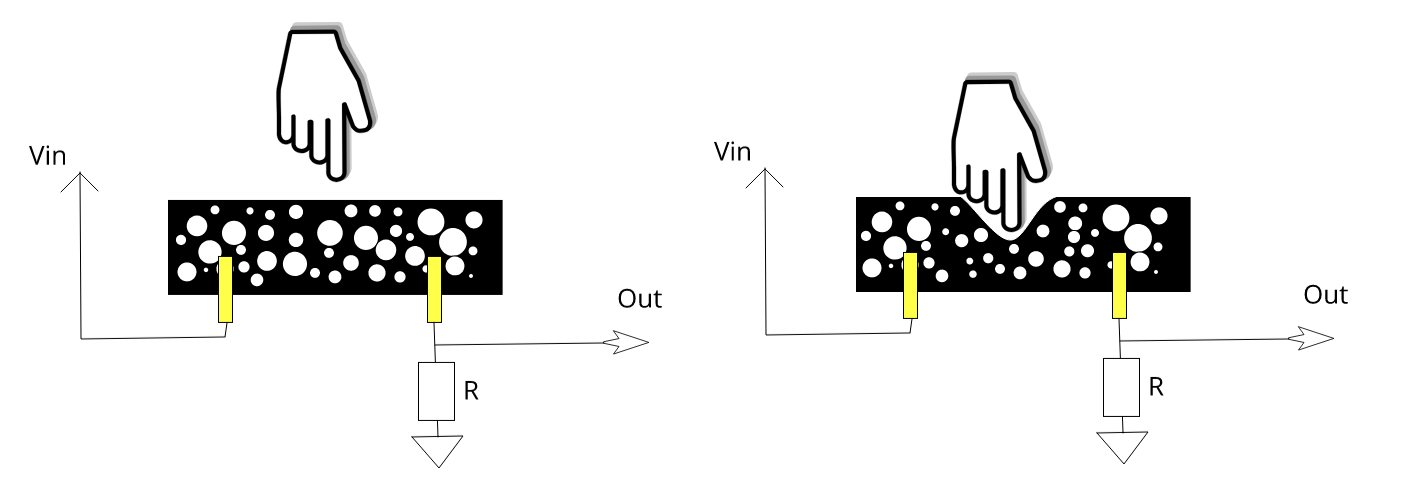
\includegraphics[width=\textwidth]{img/foam_howto.png}
    \end{center}
    % #doc .NH
    % #doc How it works
    % #doc .PP
    % #doc How this works on a high abstraction is do tho three properties of the material.
    % #doc Firstly the material have a given resistance per meter.
    % #doc Secondly the material have empty holes.
    % #doc Third. Because the material is a foam the material could be squeezed
    % #doc thus short circuit the material the resistance is changing.
\end{frame}

\begin{frame}
    \frametitle{What was done}
    \begin{center}
        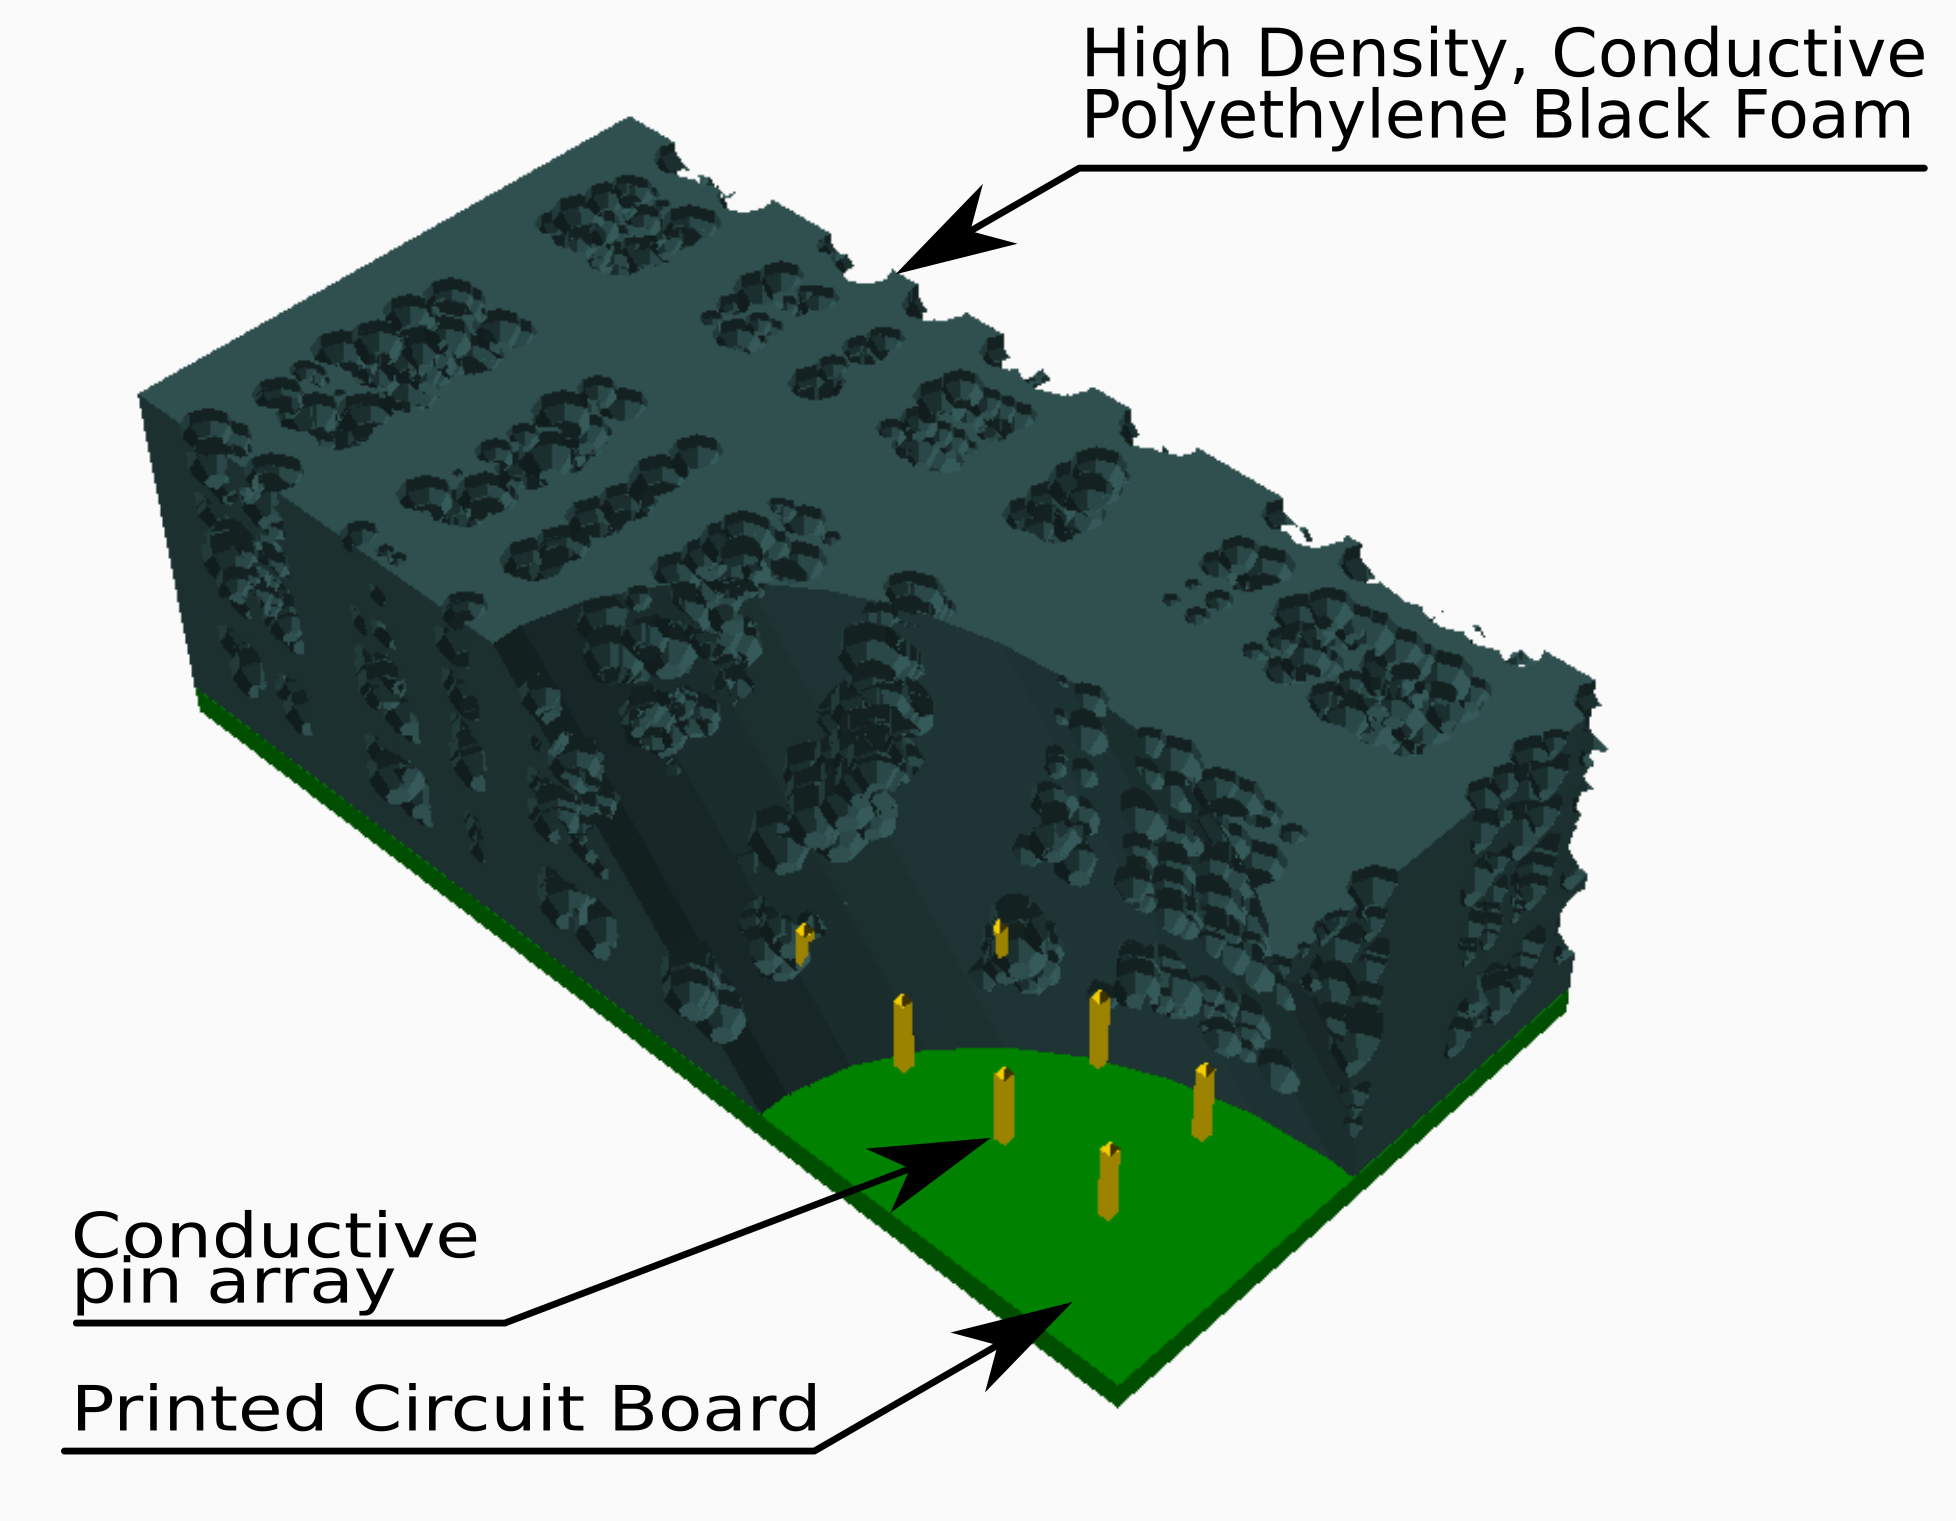
\includegraphics[width=.8\textwidth]{img/sensor_with_arrows_and_text.png}
    \end{center}
    % #doc .NH
    % #doc What was done
    % #doc .PP
    % #doc The approach to measure this is based an grid array of measurement pins inserted in to the bottom
    % #doc of the foam.
\end{frame}

\begin{frame}
    \frametitle{What was done}
    \begin{center}
        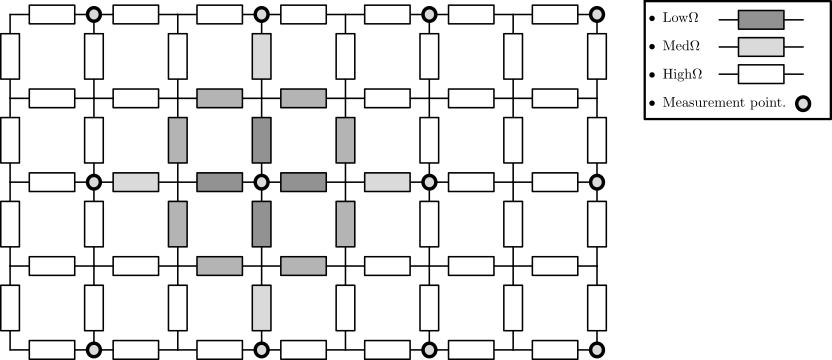
\includegraphics[width=.8\textwidth]{img/resistor_mapp_modell.png}
    \end{center}
    % #doc .PP
    % #doc That grid of measurement pins in the foam could be abstracted down to a resistor map as shown.
    % #doc In the implementation as shown later the pins in this map will be altering from positive to negative.
    % #doc And by the implemented algorithm a image of the features in the pressed down figure could be shown.
\end{frame}

\begin{frame}
    \frametitle{The algorithm}
    \begin{center}
        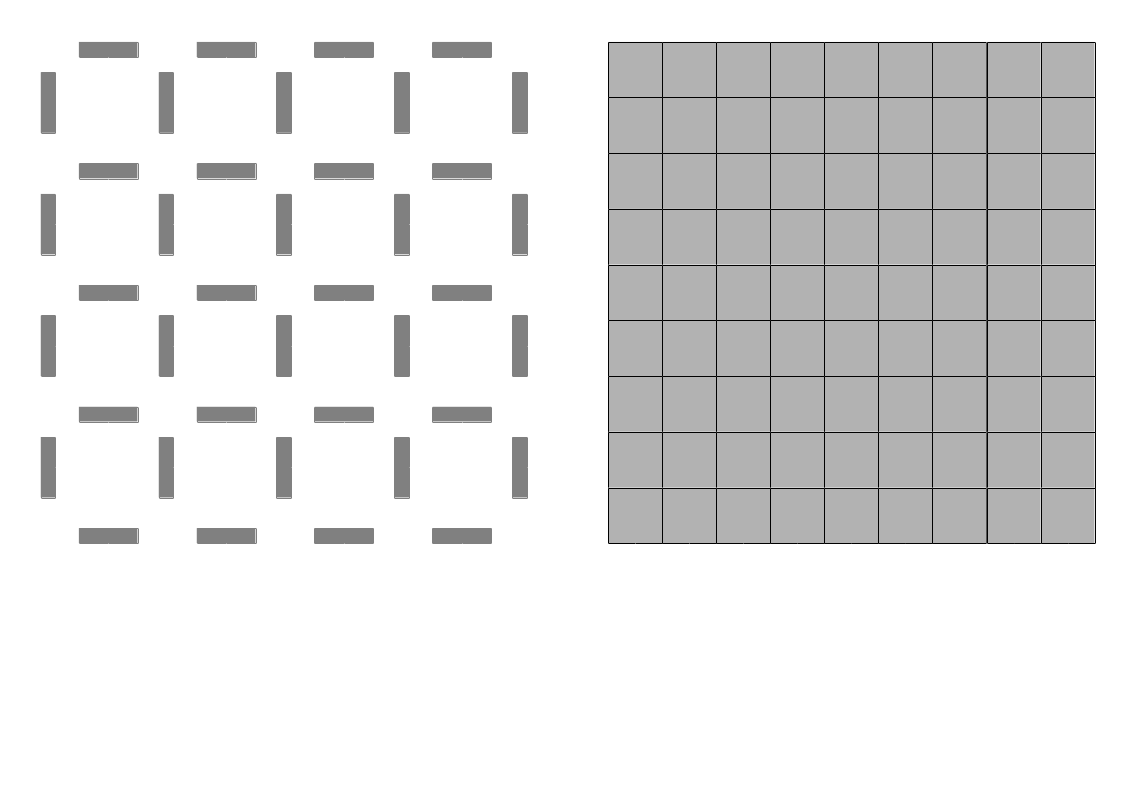
\includegraphics[width=.8\textwidth]{img/grid0.png}
    \end{center}
    % #doc .NH
    % #doc How the algorithm works
    % #doc .PP

\end{frame}

\begin{frame}
    \frametitle{The algorithm}
    \begin{center}
        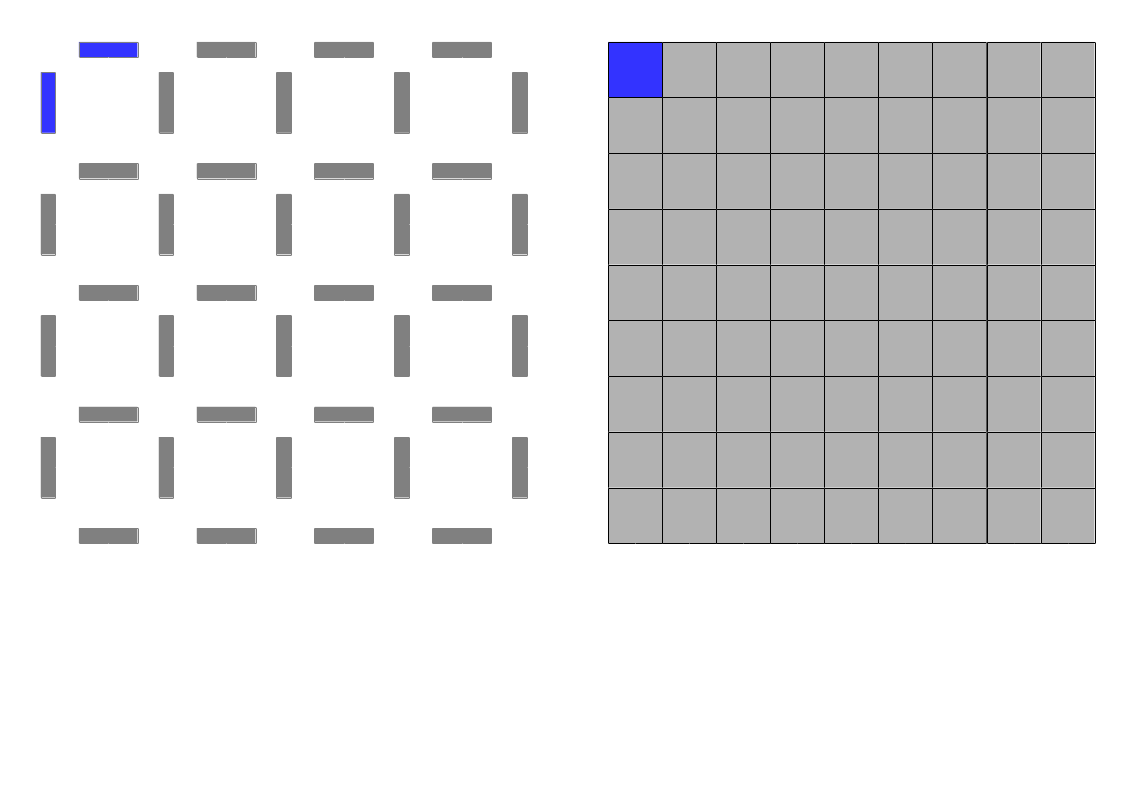
\includegraphics[width=.8\textwidth]{img/grid1.png}
    \end{center}
\end{frame}
\begin{frame}
    \frametitle{The algorithm}
    \begin{center}
        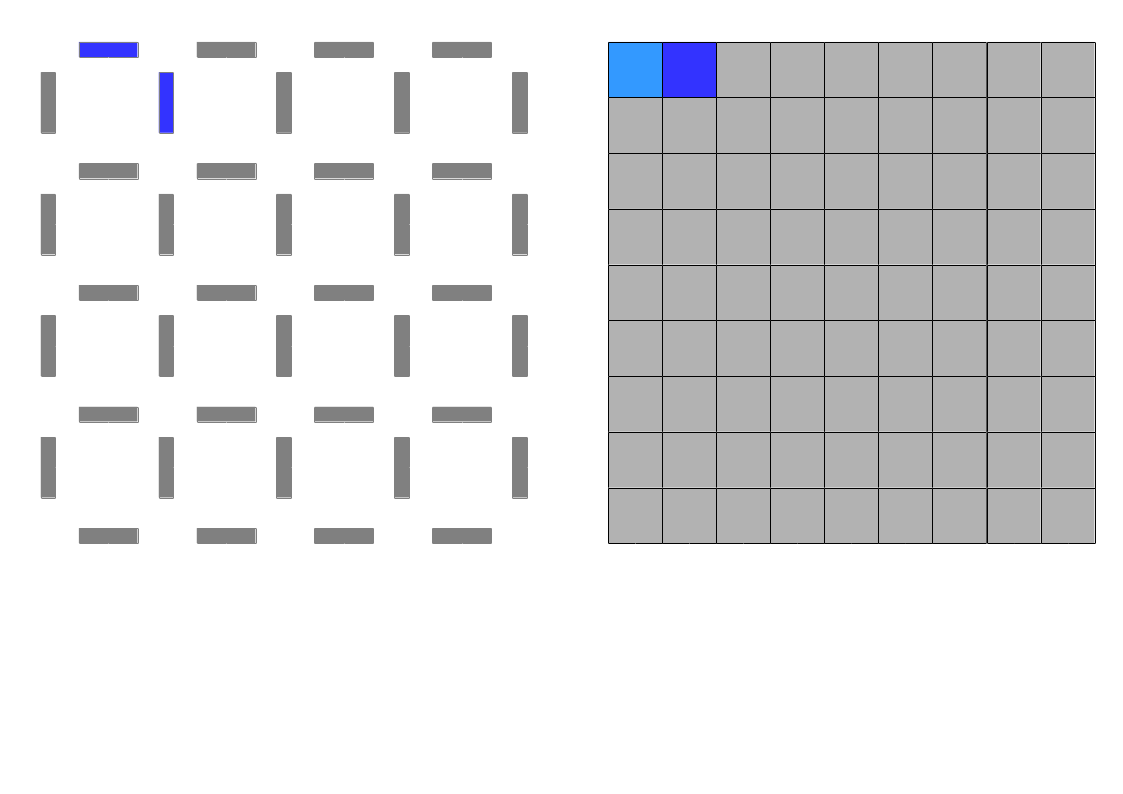
\includegraphics[width=.8\textwidth]{img/grid2.png}
    \end{center}
\end{frame}
\begin{frame}
    \frametitle{The algorithm}
    \begin{center}
        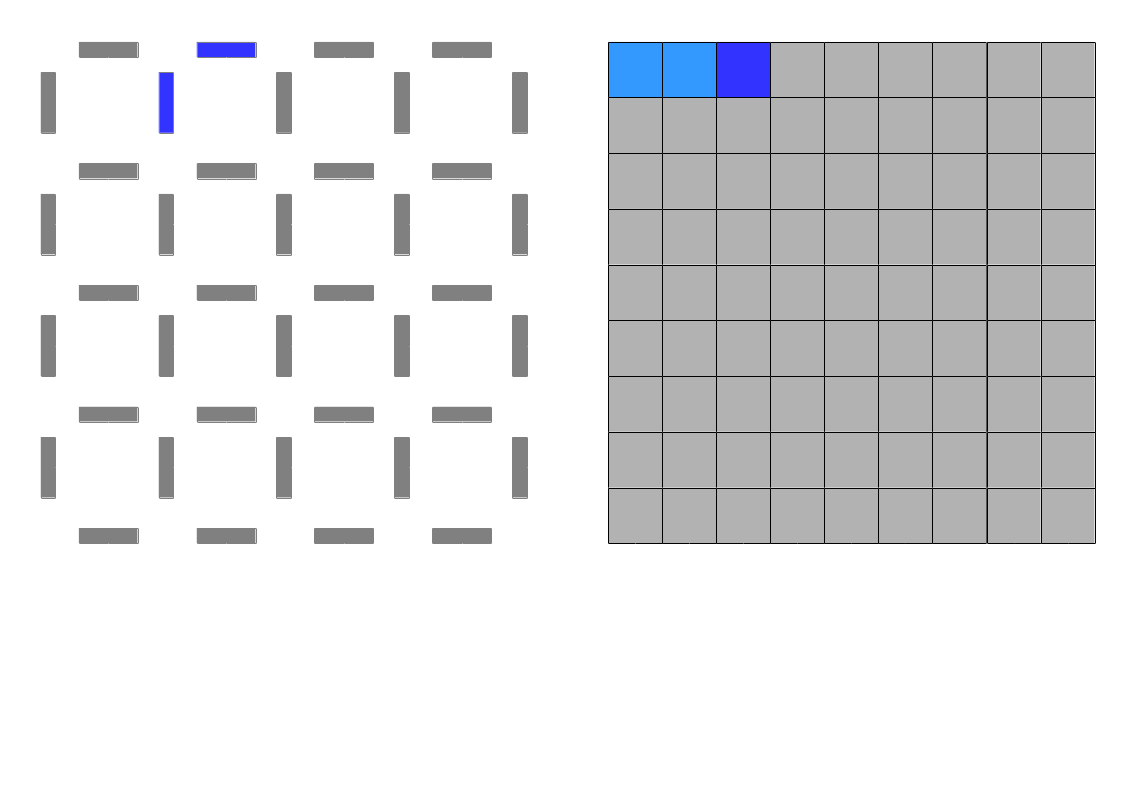
\includegraphics[width=.8\textwidth]{img/grid3.png}
    \end{center}
\end{frame}

\begin{frame}
    \frametitle{The algorithm}
    \begin{center}
        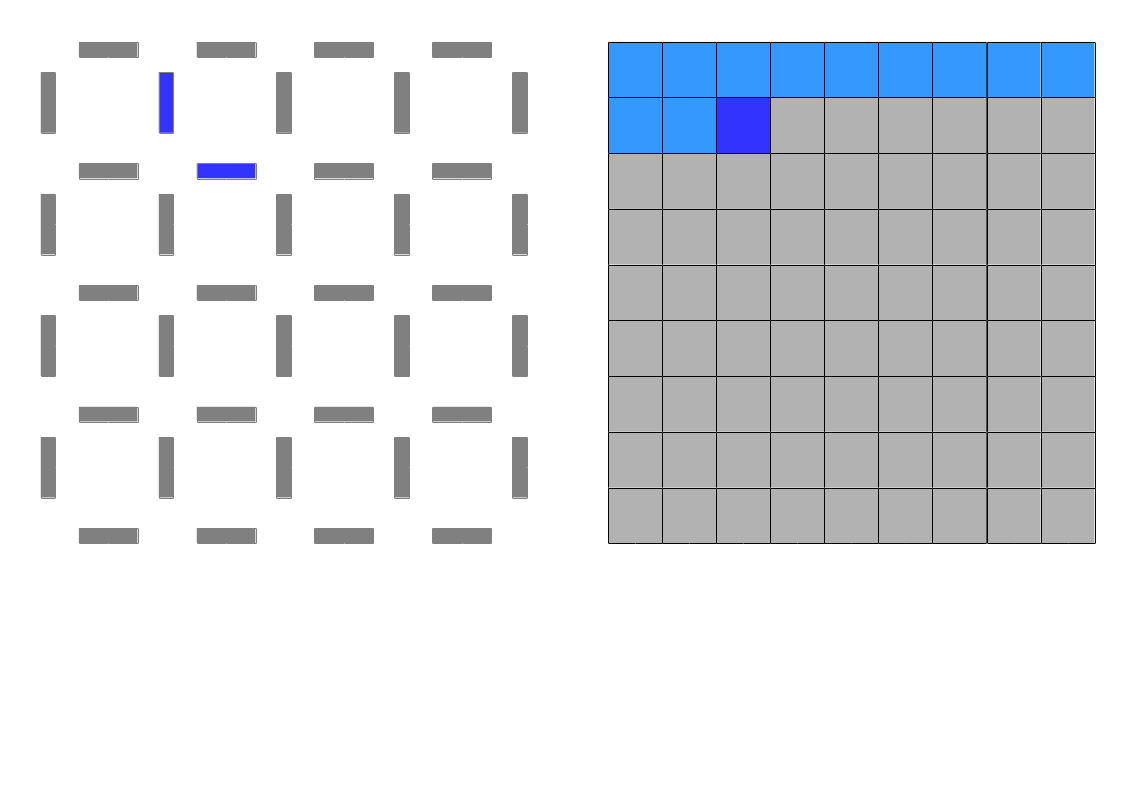
\includegraphics[width=.8\textwidth]{img/grid4.png}
    \end{center}
\end{frame}

\begin{frame}
    \frametitle{The algorithm}
    \begin{center}
        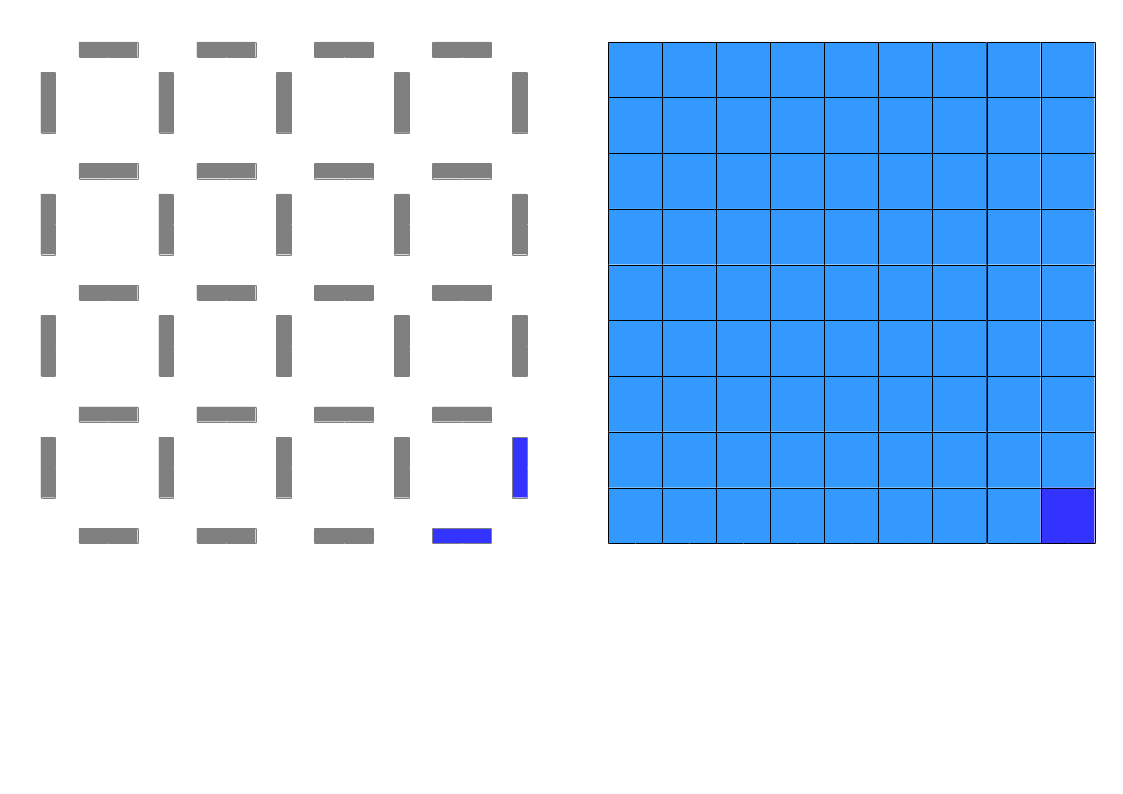
\includegraphics[width=.8\textwidth]{img/grid8.png}
    \end{center}
\end{frame}
\end{document}


